\section{Piecewise linear functions on multilevel
  grids in 2D}\label{sec:functions}
An image can be viewed as a function on a grid.  Images with different
resolutions can then be viewed as functions on grids of different
sizes.  The use of such multiple-grids is a main technique used in the
standard multigrid method for solving discretized partial differential
equations, and it can also be interpreted as a main ingredient used in
convolutional neural networks (CNN) for image calssification.

An image can be viewed as a function on a grid \cite{krizhevsky2012imagenet} on 
a rectangle  domain $\Omega\in \mathcal R^2$.  Without loss of generality,
 we assume that the grid, $\mathcal T$, is of size
$$
m=2^{s}+1~~~n=2^{t}+1 
$$
for some integers $s, t\ge 1$.
Starting from $\mathcal T_1=\mathcal T$,  we consider a sequence of
coarse grids with $J=\min (s,t)$ (as depicted in Fig.~\ref{mgrid} with $J=4$):
\begin{equation}
\label{grids}
\mathcal T_1, \mathcal T_2, \ldots, \mathcal T_J
\end{equation}
such that ${\cal T}_\ell$ consist of $m_\ell\times n_\ell$ grid
points, with 
\begin{equation}
\label{mn-ell}
 m_\ell=2^{s-\ell+1}+1,~~ n_\ell=2^{t-\ell+1}+1.   
\end{equation}
\begin{figure}[!htbp]\label{mgrid}
	\begin{center}
		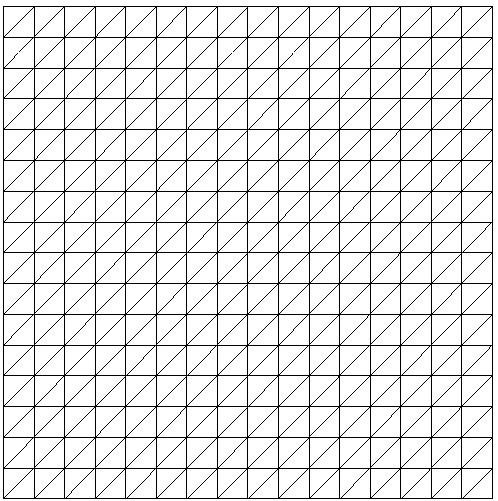
\includegraphics[width=0.15\textwidth]{grid2.png} \quad 
		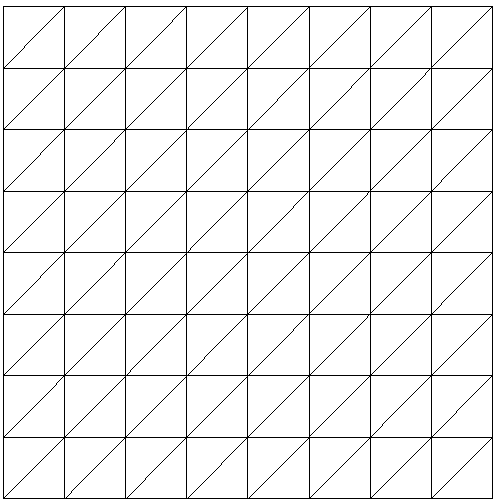
\includegraphics[width=0.15\textwidth]{grid1.png} \quad 
		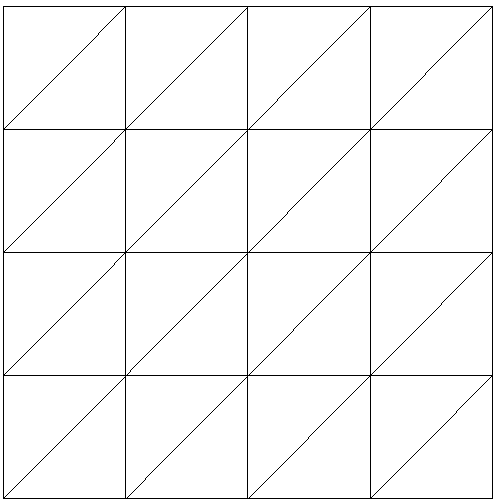
\includegraphics[width=0.15\textwidth]{grid0.png} \quad 
		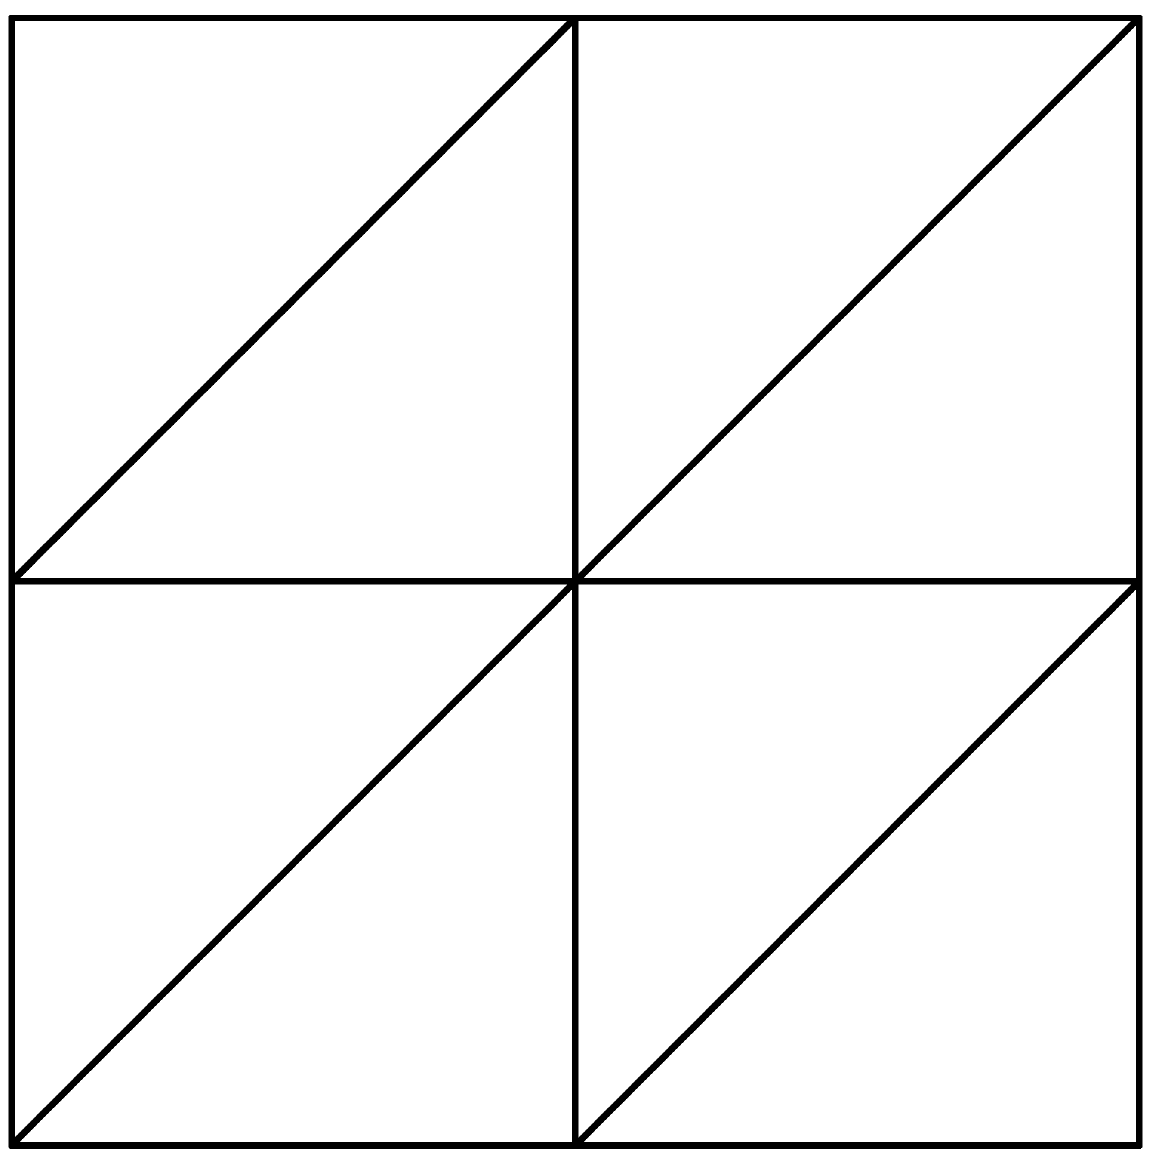
\includegraphics[width=0.15\textwidth]{grid.png} 
	\end{center}
	$$ 
\hskip0.05 in \mathcal T_1\hskip 0.7in \mathcal T_2\hskip 0.7in  \mathcal T_3\hskip 0.7in \mathcal T_4
	$$
	\caption{multilevel grids for piecewise linear functions}
\end{figure}




The grid points of these grids can be given by
$$
x_i^{\ell}=i h_{\ell}, y_j^{\ell}=j h_{\ell},  i=0, \ldots, m_\ell-1,
j=0, \ldots, n_\ell-1.
$$
Here $h_{\ell} = 2^{-s + \ell -1}a$ for some $a >0$. The above geometric coordinates $(x_i^\ell, y_j^\ell)$
are usually not used in image precess literatures, but they are relevant
in the context of multigrid method for numerical solution of PDEs.
We now consider piecewise bilinear (or linear) functions on the sequence of grids
\eqref{grids} and we obtain a nested sequence of linear vector spaces
\begin{equation}
\label{Vk}
\mathcal V_1\supset\mathcal V_2\supset\ldots\supset \mathcal
V_J.
\end{equation}




